\documentclass[landscape]{article}
\usepackage[paperwidth=42in,paperheight=24in,margin=0.65in]{geometry}
\usepackage[utf8]{inputenc}
\usepackage[T1]{fontenc}
\usepackage[spanish,es-noquoting]{babel}
\usepackage{amsmath,amssymb}
\usepackage{graphicx}
\usepackage{xcolor}
\usepackage{multicol}
\usepackage{booktabs}
\pagestyle{empty}
\graphicspath{{../figures/}}

\definecolor{ink}{HTML}{17212B}
\definecolor{accent}{HTML}{1F6F8B}
\definecolor{soft}{HTML}{EEF6F8}

\newcommand{\panel}[2]{%
  \fcolorbox{accent}{soft}{%
    \begin{minipage}[t]{0.31\textwidth}
      {\color{accent}\LARGE\bfseries #1}\par\vspace{0.35cm}
      \large #2
      \vspace{0.35cm}
    \end{minipage}}
}

\begin{document}
\color{ink}

\begin{center}
{\Huge\bfseries Ruptura de Simetría y Predicción Temprana de Especialización Axial}\\[0.25cm]
{\LARGE \emph{Seeking the Unicorn} como problema de teoría de grafos}\\[0.15cm]
{\Large Thomas Chisica · Universidad del Rosario · Teoría de Grafos 2026-I · Entrega final Codex}
\end{center}

\vspace{0.45cm}

\panel{Pregunta}{
Dos jugadores exploran una grilla $8\times8$ sin comunicación. El trabajo pregunta si la geometría del tablero ayuda a explicar y anticipar la aparición de roles espaciales axiales.
}
\hfill
\panel{Modelo}{
El tablero con conectividad de rey se modela como $P_8\boxtimes P_8$: 64 vértices y 210 aristas. Su simetría cuadrada induce $\lambda_2=\lambda_3\approx0{,}4164$.
}
\hfill
\panel{Herramienta}{
Pipeline reproducible en Python: construcción del grafo, análisis espectral, particiones humanas, conductancia, MI/JSD, robustez temporal y predicción temprana.
}

\vspace{0.55cm}

\begin{minipage}[t]{0.32\textwidth}
{\color{accent}\Huge\bfseries Resultado estructural}\par
\vspace{0.25cm}
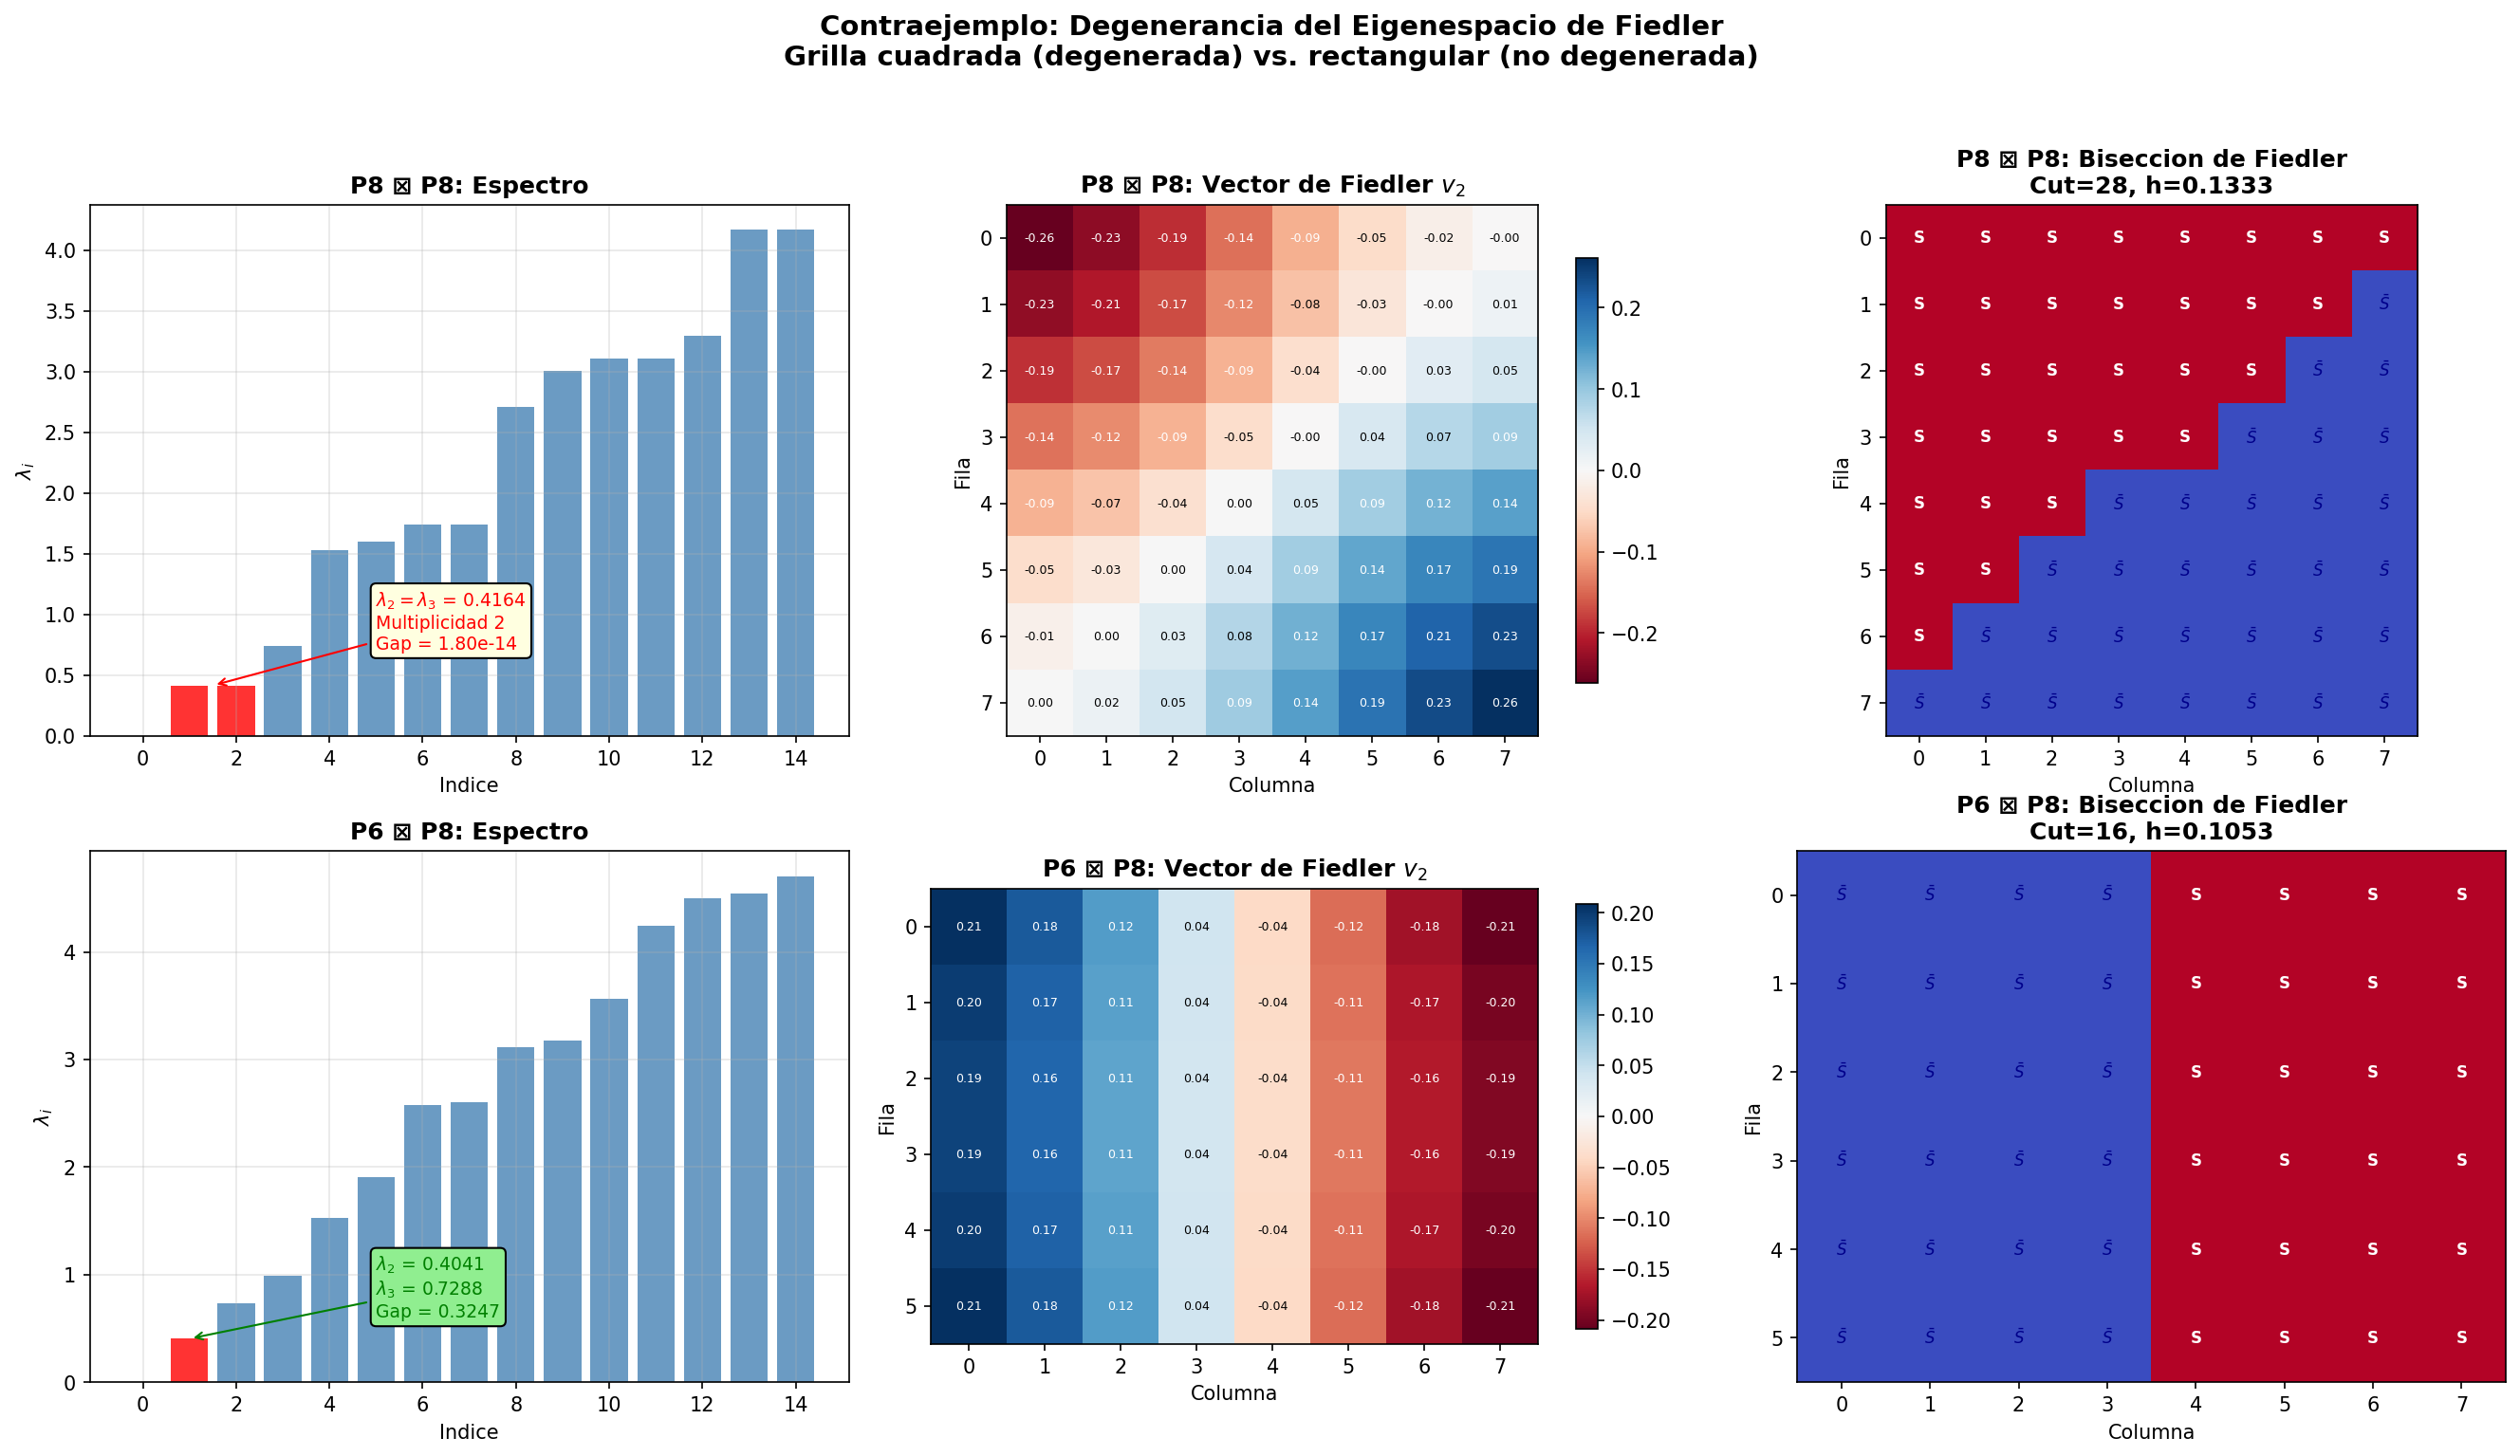
\includegraphics[width=\textwidth]{counterexample_P6xP8.png}
\large
El caso cuadrado produce un eigenespacio de Fiedler degenerado; al pasar a un rectángulo, la degeneración se rompe. Esto explica por qué un único vector de Fiedler no es un baseline canónico.
\end{minipage}
\hfill
\begin{minipage}[t]{0.32\textwidth}
{\color{accent}\Huge\bfseries Separación axial/mixta}\par
\vspace{0.25cm}
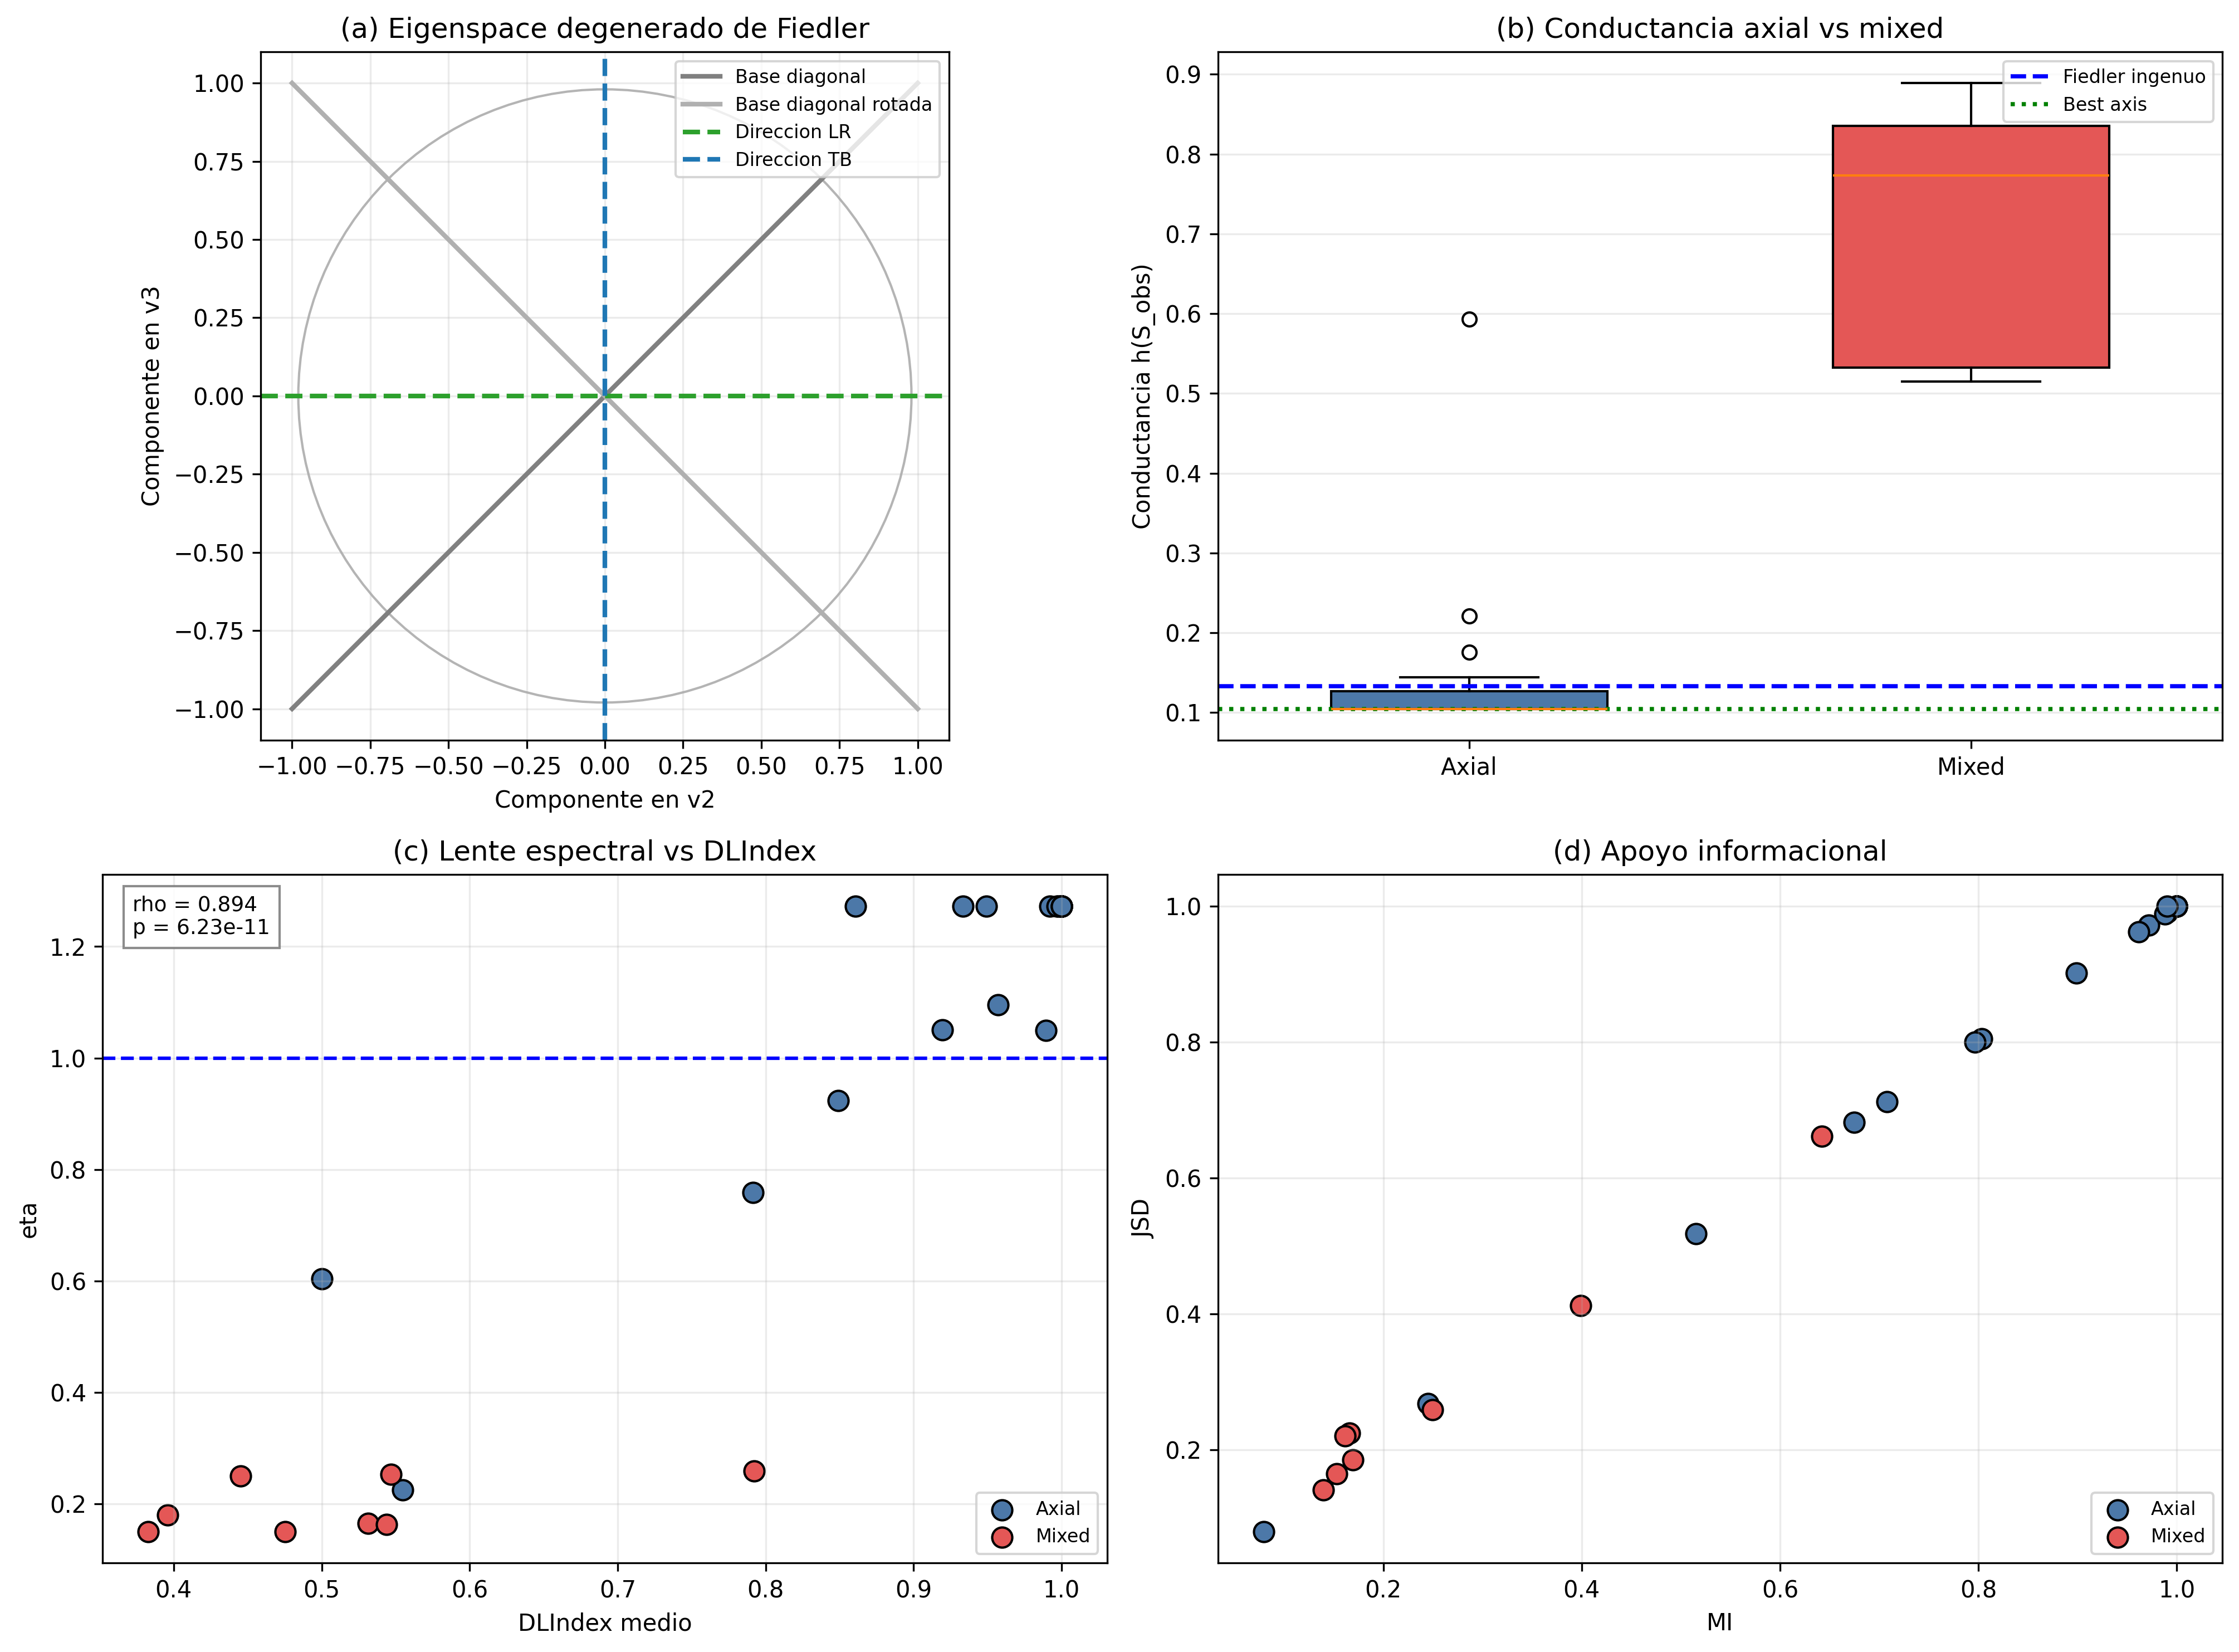
\includegraphics[width=\textwidth]{andrade_summary.png}
\large
En el set primario, 21 díadas axiales tienen menor conductancia y mayor especialización informacional que 8 díadas mixtas. El resultado es fuerte descriptivamente, pero parcial.
\end{minipage}
\hfill
\begin{minipage}[t]{0.32\textwidth}
{\color{accent}\Huge\bfseries Predicción temprana}\par
\vspace{0.25cm}
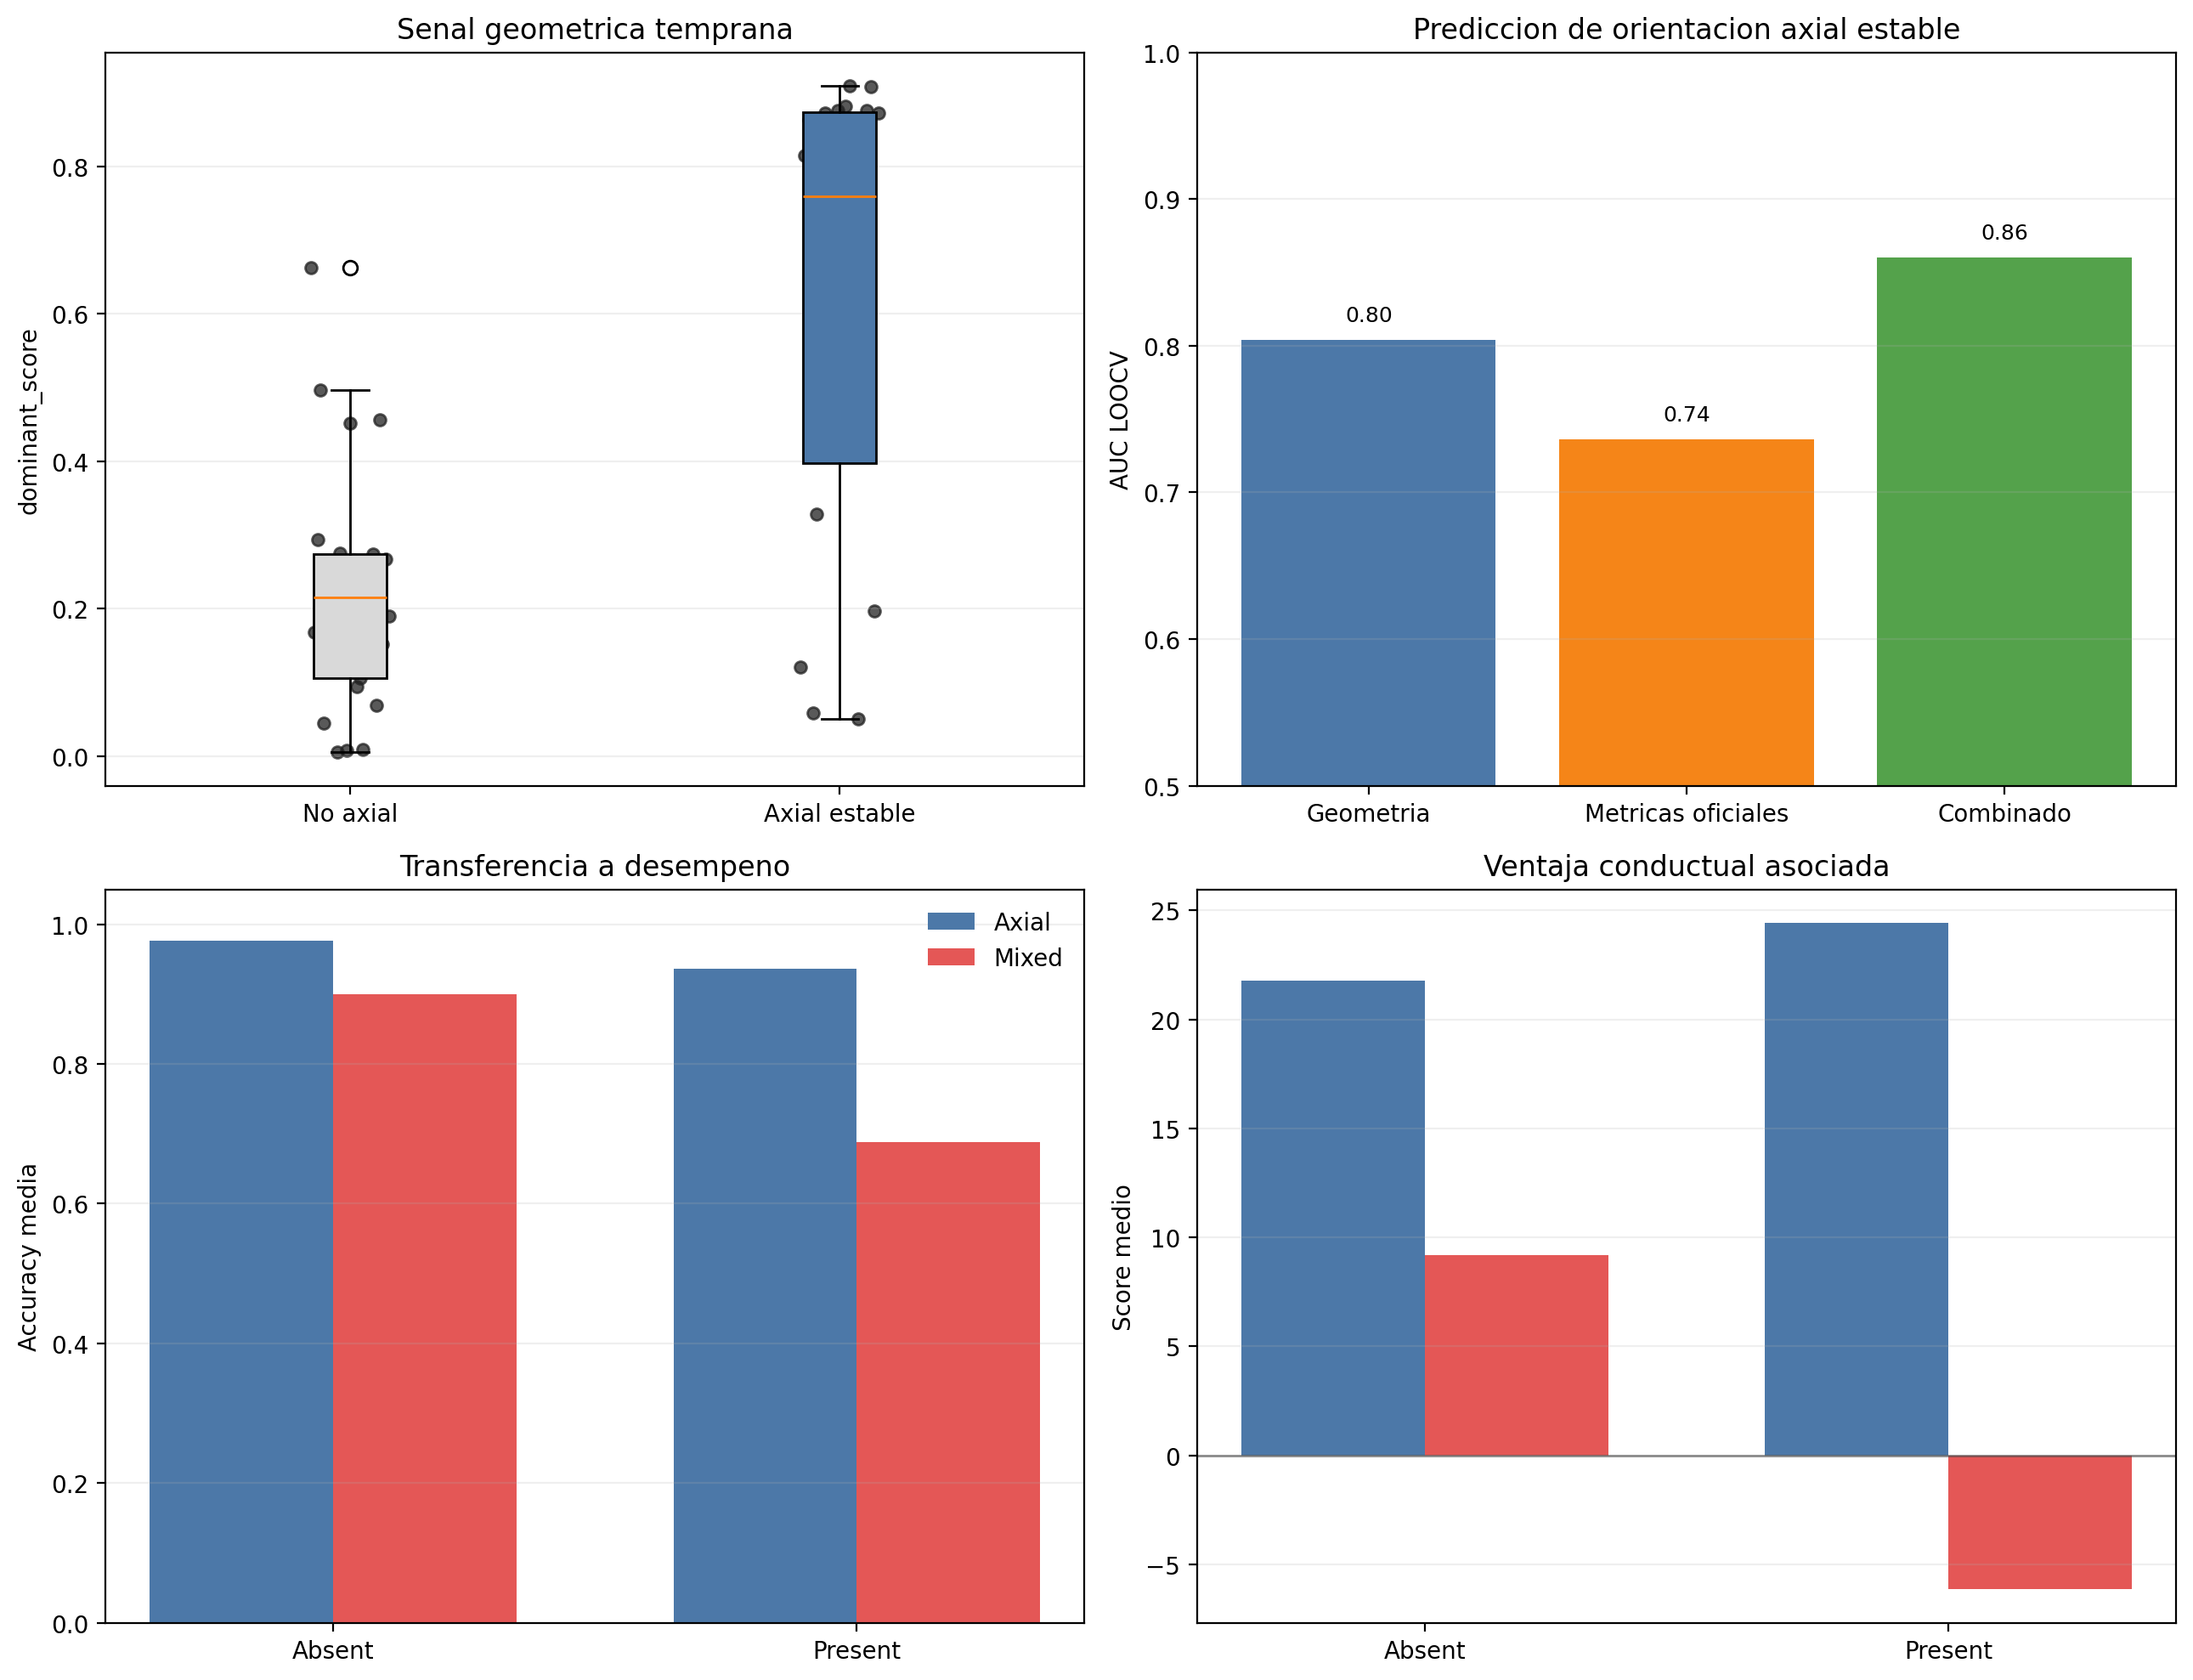
\includegraphics[width=\textwidth]{early_prediction_summary.png}
\large
Con las primeras cinco rondas ausentes, la señal geométrica alcanza AUC LOOCV $0{,}804$; métricas oficiales tempranas, $0{,}736$; modelo combinado, $0{,}860$.
\end{minipage}

\vspace{0.65cm}

\begin{minipage}[t]{0.48\textwidth}
{\color{accent}\Huge\bfseries Conclusión}\par
\Large
La contribución no es afirmar que los humanos optimizan conductancia. La contribución es mostrar que la simetría del grafo induce direcciones axiales privilegiadas y que una señal temprana de alineación geométrica ayuda a anticipar la especialización posterior.
\end{minipage}
\hfill
\begin{minipage}[t]{0.48\textwidth}
{\color{accent}\Huge\bfseries Trabajo futuro}\par
\Large
La predicción experimental natural es romper la simetría: tableros rectangulares u obstáculos deberían reducir la ambigüedad LR/TB y cambiar la distribución de convenciones humanas.
\end{minipage}

\end{document}
